%=================AVANCES Y PRUEBAS=================
% SENSORES DE PULSO

\section{Módulo Datos Personales}
Para que el usuario pueda consultar sus datos personales es necesario que siga el flujo establecido, el cual se describe a continuación.\\


\subsection{Consulta Datos Personales}

La figura \ref{fig:SecuenciaDatosPersonales} se muestra el diagrama de secuencia correspondiente al login del usuario, mismo que contiene los métodos implementados en la clase JAVA, API e IU.

\begin{figure}[htbp!]
	\centering
	\fbox{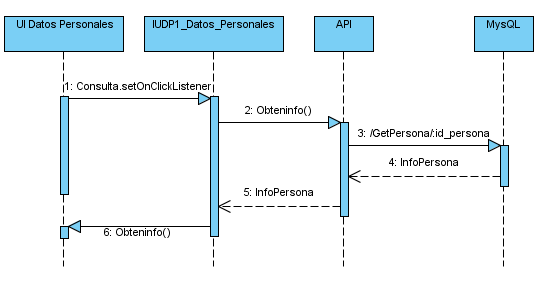
\includegraphics[width=0.9\textwidth]{AvancesPruebas/imagenes/SecuenciaInfoPersona}}
	\caption{Diagrama secuencia Consulta Datos Personales}
	\label{fig:SecuenciaDatosPersonales}
\end{figure}
\begin{itemize}
	\item \textbf{Consulta.setOnClickListener:} Es la acción que dispara el usuario, no recibe datos como parámetros, es el disparador.
	\item \textbf{Obteninfo():} Es el método que hace la llamada al API para obtener la info del usuario.
	\item \textbf{/GetPersona/:id persona:} Es la ruta para la obtención de la información de los datos del usuario.
\end{itemize}

\subsection{Consulta Datos Cuenta}

La figura \ref{fig:SecuenciaInfoCuenta} se muestra el diagrama de secuencia correspondiente al login del usuario, mismo que contiene los métodos implementados en la clase JAVA, API e IU.

\begin{figure}[htbp!]
	\centering
	\fbox{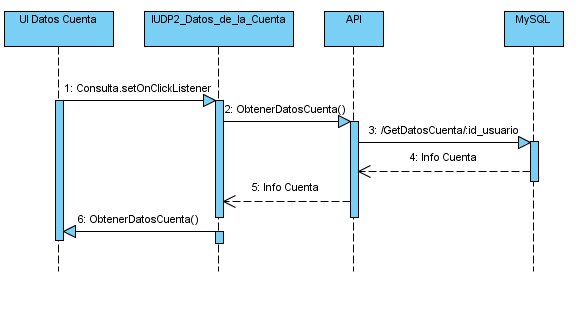
\includegraphics[width=0.9\textwidth]{AvancesPruebas/imagenes/SecuenciaInfoCuenta}}
	\caption{Diagrama secuencia Consulta Datos de Cuenta}
	\label{fig:SecuenciaInfoCuenta}
\end{figure}

\begin{itemize}
	\item \textbf{Consulta.setOnClickListener:} Es la acción que dispara el usuario, no recibe datos como parámetros, es el disparador.
	\item \textbf{ObtenerDatosCuenta():} Es el método que hace la llamada al API para obtener la info de la cuenta.
	\item \textbf{/GetDatosCuenta/:id usuario:} Es la ruta para la obtención de la información de los datos de la cuenta.
\end{itemize}







